\documentclass{beamer}
\mode<presentation>
{
  \usetheme{Madrid}
  %\usetheme{Antibes}
  % or ...
  %\usecolortheme{seahorse}
  \setbeamercovered{transparent}
  % or whatever (possibly just delete it)
}


\usepackage[english]{babel}
\usepackage[latin1]{inputenc}
\usepackage{times}
\usepackage[T1]{fontenc}
\usepackage{subfigure}
\usepackage{multirow}
\usepackage{hyperref}
\usepackage{epstopdf}
\usepackage{color}% This package is for using color package.
\newcommand{\red}[1]{\textcolor{red}{#1}}% Chang-Dong uses red text to state the revision or revision note.
\title[MVIR] % (optional, use only with long paper titles)
{An Item Orientated Recommendation from Multi-view Perspective}

\author[Hu \emph{et al.}] % (optional, use only with lots of authors)
{Qi-Ying Hu\inst{1} \and Zhi-Lin Zhao\inst{1}\\
\and Chang-Dong Wang\inst{1}
\and Jian-Huang Lai\inst{1}}%

\institute[Sun Yat-sen University] % (optional, but mostly needed)
{
  \inst{1}%
  School of Data and Computer Science\\
  Sun Yat-sen University, P. R. China.
}

%\author[Wang \emph{et al.}] % (optional, use only with lots of authors)
%{Chang-Dong Wang \and Jian-Huang Lai\\
%\and Jun-Yong Zhu}%
%
%\institute[Sun Yat-sen University] % (optional, but mostly needed)
%{Sun Yat-sen University, P. R. China}


\date[IScIDE 2016] % (optional, should be abbreviation of conference name)
{The 2016 International Conference on Intelligence Science and Big Data Engineering}

% Delete this, if you do not want the table of contents to pop up at
% the beginning of each subsection:
%\AtBeginSubsection[]
%{
%  \begin{frame}<beamer>
%    \frametitle{Outline}
%    \tableofcontents[currentsection,currentsubsection]
%  \end{frame}
%}

\begin{document}

\begin{frame}
  \titlepage
  
\includegraphics[width=0.18\linewidth]{Figures/Sysu_logo}
\end{frame}

\begin{frame}
  \frametitle{Outline}
  \tableofcontents%[pausesections]
  % You might wish to add the option [pausesections]
\end{frame}


% Structuring a talk is a difficult task and the following structure
% may not be suitable. Here are some rules that apply for this
% solution:

% - Exactly two or three sections (other than the summary).
% - At *most* three subsections per section.
% - Talk about 30s to 2min per frame. So there should be between about
%   15 and 30 frames, all told.

% - A conference audience is likely to know very little of what you
%   are going to talk about. So *simplify*!
% - In a 20min talk, getting the main ideas across is hard
%   enough. Leave out details, even if it means being less precise than
%   you think necessary.
% - If you omit details that are vital to the proof/implementation,
%   just say so once. Everybody will be happy with that.

\section{Motivation}
\subsection{Background}
\begin{frame}
\frametitle{Traditional Recommendation Algorithms}
%\begin{itemize}
%\item
%In the traditional recommendation algorithms%, items are recommended to users on the basis of users' preferences to improve selling efficiency.
%\vskip 0.4in
%\item However, all the existing algorithms \red{only take the users benefits into consideration}, and there are \red{no} algorithms designed to raise revenues for the manufacturer of a particular item.

%\end{itemize}
\begin{figure}[!t]
\renewcommand{\subfigcapskip}{-4pt}
\renewcommand{\subfigbottomskip}{0pt}
\centering
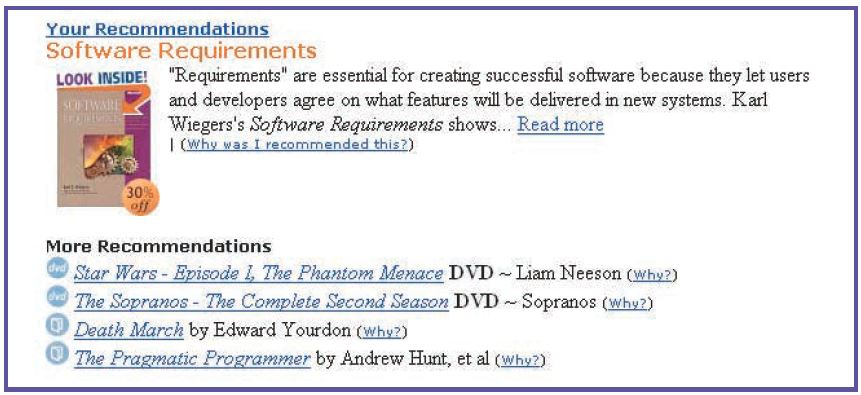
\includegraphics[width=0.6\linewidth]{Figures/Recommendation}
\caption{Recommendation based on user's preference.}
\label{fig:Recommendation}
%\vskip -0.2in
\end{figure}

\begin{figure}[!t]
\renewcommand{\subfigcapskip}{-4pt}
\renewcommand{\subfigbottomskip}{0pt}
\centering
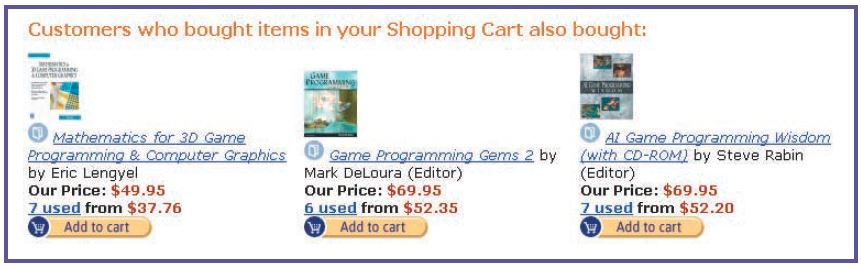
\includegraphics[width=0.6\linewidth]{Figures/Recommendation1}
\caption{Recommendation based on user's purchasing history.}
\label{fig:Recommendation1}
%\vskip -0.2in
\end{figure}
\end{frame}
\subsection{Problem Definition}
\begin{frame}
\frametitle{Problem Definition}
\begin{itemize}
\item Assume that, a manufacturer has a \red{limited budget} for an item's advertisement. With this budget, it is only possible for him to market this item to the limited number of users.
\vskip 0.4in
\item How to select the most suitable users that will maximize the advertisement benefits?
\vskip 0.4in
\item To address the above issue, we present an approach based on the \red{multi-view learning} and perform \red{item orientated recommendation}.
\end{itemize}
\end{frame}
\section{The Proposed Model - MVIR}
\subsection{The Multi-view Model}
\begin{frame}
\frametitle{The Multi-view Model}
The rating records of each user are taken as a view where the items rated by the user can be represented as nodes.%and there exists an edge between any pair of nodes with the weight of edge being the relationship between two items w.r.t. the user.
\vskip 0.2in
\begin{itemize}
\item \textbf{Within-view Relationship}: The item relationship computed in an individual view, depicting the relationship between items revealed by the single user.
\vskip 0.2in
\item \textbf{Cross-view Relationship}: The edge between items across different views, simultaneously considering both the consistency and diversity of item preferences among different users.
\end{itemize}
\end{frame}

\begin{frame}
\frametitle{The Multi-view Model}
\begin{figure}[!t]
\renewcommand{\subfigcapskip}{-4pt}
\renewcommand{\subfigbottomskip}{0pt}
\centering
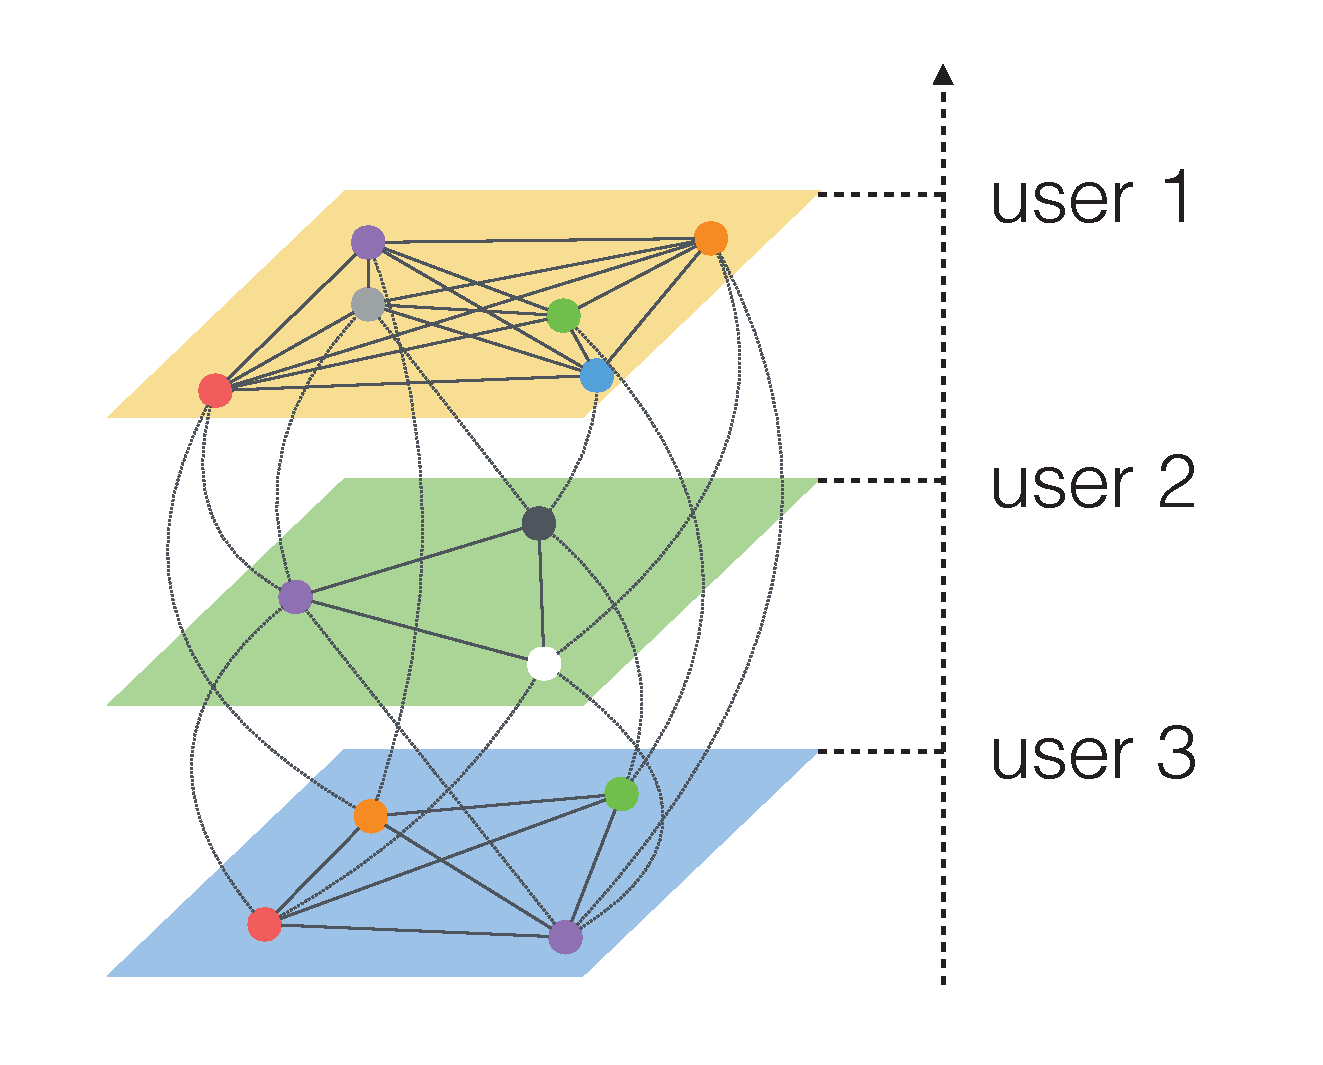
\includegraphics[width=0.6\linewidth]{Figures/Multiview.eps}
\caption{Within-view relationship and cross-view relationship in multi-view model.}
\label{fig:Multiview}
%\vskip -0.2in
\end{figure}
\end{frame}

\begin{frame}
\frametitle{Within-View and Cross-View Relationships}
Given a user-item rating matrix $R=[r_{u,i}]_{M \times N}$, whose two dimensions correspond to user and item with sizes $M$ and $N$, respectively. Each entry $r_{u,i}$ %of $R$ in row $u$ and column $i$
denotes the rating of user $u$ to item $i$.

\begin{enumerate}
\item Within-view relationship:\\
Different items $i$ and $j$ %in an individual view
corresponding to user $u$, denoted as $S^u_{i,j}$:
\begin{equation}\label{eq:within_view}
  S^u_{i,j} = \sqrt{r_{u,i}^2+r_{u,j}^2}.
\end{equation}
\item Cross-view relationship:\\
Item {$i$} purchased by user $u$ and item $j$ purchased by user $v$, %across two different views corresponding to user $u$ and user $v$,
denoted as $S^{u,v}_{i,j}$:
\begin{equation}\label{eq:cross_view}
  S^{u,v}_{i,j} = \sqrt{r_{u,i}^2+r_{v,j}^2}.
\end{equation}
\end{enumerate}
\end{frame}

\begin{frame}
\frametitle{Within-View and Cross-View Relationships}
\begin{figure}[!t]
\renewcommand{\subfigcapskip}{-4pt}
\renewcommand{\subfigbottomskip}{0pt}
\centering
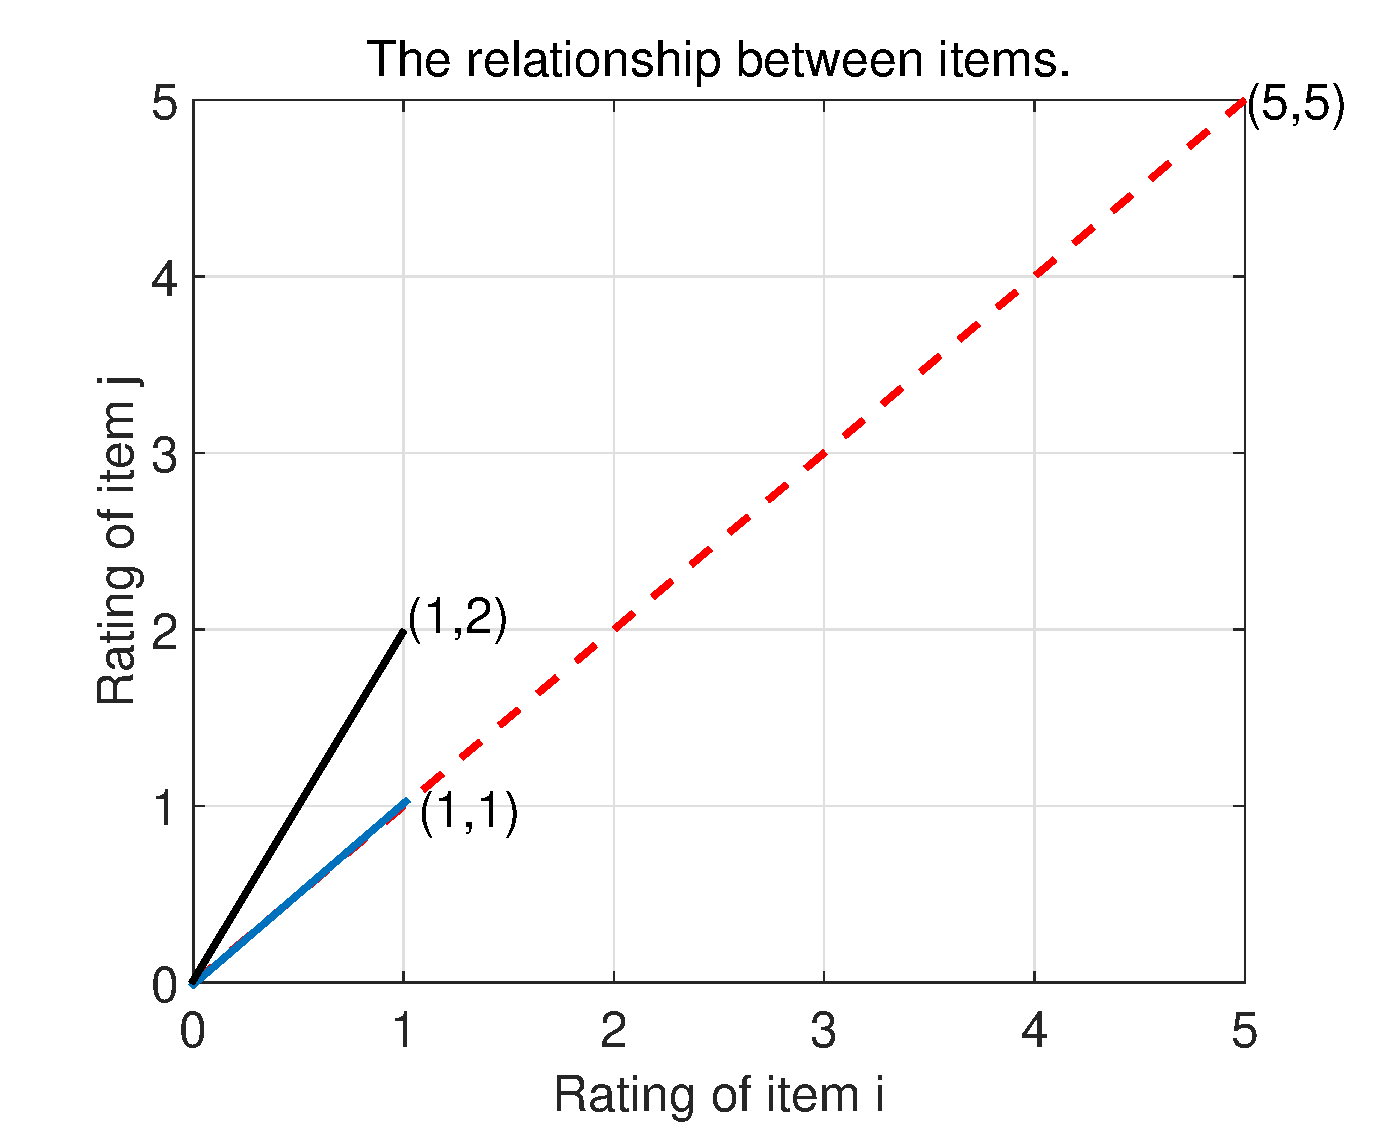
\includegraphics[width=0.6\linewidth]{Figures/Relationship.eps}
\caption{The relationship between items. We define that only when \red{two items have high ratings and the ratings of them are similar}, the value of relationship will be higher and the items are closer.}
\label{fig:Relationship}
%\vskip -0.2in
\end{figure}
\end{frame}
\subsection{Objection Function}
\begin{frame}
\frametitle{Objection Function}
\begin{itemize}
  \item<2->
The goal of the multi-view model is tolearn the \red{relationship matrix $\alpha$} and the \red{rating difference matrix $\beta$}.

\begin{itemize}
\item \textbf{$\alpha$}: The entry $\alpha_{i,j}$, representing the relationship between items, is consistent both in an individual view and multi view.
\vskip 0.2in
\item \textbf{$\beta$}:  The entry $\beta_{u,v}$ represents the rating difference between users.
\end{itemize}

\vskip 0.2in
  \item<3->
The objective function can be written as follows.
\begin{equation}\label{eq:objectivefunction}
\begin{aligned}
  & \alpha,\beta = \arg\min_{\alpha,\beta} E = \arg\min_{\alpha,\beta} \delta \sum^M_{u=1}\quad\sum^N_{i,j \in \mathcal{N}_(u), i < j} \left( \alpha_ {i,j}-S^u_{i,j}\right)^2 \\
  & + \left(1-\delta\right) \sum^M_{u=1,{v=2},u<v}\quad \sum^N_{i \in \mathcal{N}_(u), j \in \mathcal{N}_(v), i<j}\left(\alpha_{i,j} - S^{u,v}_{i,j}-\beta_{u,v}\right)^2\;  .
\end{aligned}
\end{equation}
\end{itemize}
\end{frame}

\subsection{Model Optimization}
\begin{frame}
\frametitle{Model Optimization}

%\begin{itemize}
%  \item<2->
We can use the \red{gradient descent method} to get the solution of the above function:
\begin{equation}
\begin{aligned}\label{eq:gd_alpha}
   & \nabla \alpha_{i,j} = \frac{\partial E} {\partial \alpha_{i,j}} =2 \delta \sum^M_{u=1}(\alpha_{i,j}-S^u_{i,j}) \\
   & + 2(1-\delta) \sum^M_{u=1,{v=2},u<v}(\alpha_{i,j} - S^{u,v}_{i,j}-\beta_{u,v}).
\end{aligned}
\end{equation}
\begin{equation}
\begin{aligned}\label{gd_beta}
    \nabla \beta_{u,v} = \frac{\partial E} {\partial \beta_{u,v}} = - 2(1-\delta) \sum^N_{i \in \mathcal{N}_(u), j \in \mathcal{N}_(v), i<j}(\alpha_{i,j} - S^{u,v}_{i,j}-\beta_{u,v}).
\end{aligned}
\end{equation}
\vskip 0.2in

\end{frame}

\begin{frame}
\frametitle{Model Optimization}
After computing the $\nabla \alpha_{i,j}$ and $\nabla \beta_{u,v}$, the entries in $\alpha$ and $\beta$ can be updated by the following equations {in which} $\gamma$ is the learning rate.
\vskip 0.2in
\begin{equation}
\begin{aligned}\label{update_alpha}
   \alpha_{i,j} = \alpha_{i,j} - \gamma \nabla \alpha_{i,j}.
\end{aligned}
\end{equation}
\begin{equation}
\begin{aligned}\label{update_beta}
   \beta_{u,v} = \beta_{u,v} - \gamma \nabla \beta_{u,v}.
\end{aligned}
\end{equation}
\end{frame}

\subsection{Recommend Users to Items.}
\begin{frame}
\frametitle{Recommend Users to Items.}
%By obtaining the relationship matrix $\alpha$ and rating difference matrix $\beta$, as to the target item $i$, we can implement the item orientated recommendation.
\vskip -0.2in
As to item $i$, let
\vskip 0.2in
\begin{itemize}
\item $k_1$: the number of the chosen items that are closest to $i$.
\vskip 0.2in
\item $k_2$: the number of the users recommended to $i$ who are most likely to buy the item.
\end{itemize}
\end{frame}

\begin{frame}
\frametitle{Recommend Users to Items.}
\begin{enumerate}
\item<2-> Find $k_1$ items by sorting the $i$-th row in $\alpha$.
\vskip 0.2in
\item<3-> Find two \red{disjoint sets} $h_1$ and $h_2$ that represent the users have purchased $i$ and the users have purchased at least one item in the $k_1$ items list,
\vskip 0.2in
\item<4-> $\forall u \in h_2$, compute the \red{mean of the total differences} between $u$ and all users in $h_1$. The $D_i$ set is used to record the differences of user $u$.
\vskip 0.2in
\item<5-> Sort $D_i$ according to the \red{ascending order}, find the smallest $k_2$ users. Recommend these users to item $i$.
\end{enumerate}
\end{frame}

\section{Experiment Results}
\subsection{Dataset \& Evaluation Metrics}
\begin{frame}
\frametitle{Dataset \& Evaluation Metrics}
\begin{itemize}
\item<2-> \textbf{Dataset}: The four datasets used in our experiments are \emph{BaiduMovie}, \emph{EachMovie}, \emph{Jester} and \emph{MovieLens}.
\vskip 0.2in
\item<3-> \textbf{Evaluation Metrics}: The performances of the recommendation are measured by $Precision$, $Recall$ and $F_1$.

\begin{equation}\label{eq:precision}
  Precision = \frac{\sum_i^N |R(i) \bigcap T(i)|}{\sum_i^N |R(i)|}
\end{equation}
\begin{equation}\label{eq:recall}
  Recall = \frac{\sum_i^N |R(i) \bigcap T(i)|}{\sum_i^N |T(i)|}
\end{equation}
\begin{equation}\label{eq:F_1}
  F_1 = \frac{2 \times Precision \times Recall}{Precision + Recall}
\end{equation}
where $R(i)$ is the \red{recommendation list} to the target item $i$ %computed from the training dataset
and $T(i)$ is the \red{behavior list} of item $i$ on the testing dataset.

\end{itemize}
\end{frame}
\subsection{Parameters Analysis}
\begin{frame}
\frametitle{Parameter Analysis on $\delta$}
Vary the value of $\delta$ from 0 to 0.9 with $k_1$ = 5 and $k_2$=100, and the discussions of other values of $k_1$ and $k_2$ are similar.
\begin{figure}[h]
\begin{center}
{\includegraphics[width=0.24\linewidth]{Figures/Baidu_tradeoff.eps}\label{fig:tradeoffbaidu}}
{\includegraphics[width=0.24\linewidth]{Figures/EachMovie_tradeoff.eps}\label{fig:tradeoffeachmovie}}
{\includegraphics[width=0.24\linewidth]{Figures/Jester_tradeoff.eps}\label{fig:tradeoffjester}}
{\includegraphics[width=0.24\linewidth]{Figures/MovieLens_tradeoff.eps}\label{fig:tradeoffmovielens}}
\caption{The value of metrics with different $\delta$ values on four datasets in MVIR. }
\label{fig:tradeoff}
\end{center}
\end{figure}
Apparently varying the value of $\delta$ in a interval [0,1) does not cause significant changes. Overall, \red{the performances of the MVIR algorithm are robust to the parameter $\delta$} on the four datasets.
\end{frame}

\begin{frame}
\frametitle{Parameter Analysis on $k_1$ and $k_2$}
For each dataset, we conduct the analysis of $k_1$ and $k_2$ on the value of $\delta$ that achieves the maximum recommended effects. We set $k_1$ = 5, 10, 15 and $k_2$= 100, 150, 200.
\begin{figure}[h]
\begin{center}
{\includegraphics[width=0.24\linewidth]{Figures/Baidu_k_precision.eps}\label{fig:kpbaidu}}
{\includegraphics[width=0.24\linewidth]{Figures/EachMovie_k_precision.eps}\label{fig:kpeachmovie}}
{\includegraphics[width=0.24\linewidth]{Figures/Jester_k_precision.eps}\label{fig:kpjester}}
{\includegraphics[width=0.24\linewidth]{Figures/MovieLens_k_precision.eps}\label{fig:kpmovielens}}
\caption{The value of $Precision$ with different $k_1$ and $k_2$ values on four datasets in MVIR.}
\label{fig:kp}
\end{center}
\end{figure}
Overall, the performance of the recommendation will be better when \red{the value of $k_1$ is smaller and the value of $k_2$ is larger}.
\end{frame}

\begin{frame}
\begin{figure}[h]
\begin{center}
{\includegraphics[width=0.24\linewidth]{Figures/Baidu_k_recall.eps}\label{fig:krbaidu}}
{\includegraphics[width=0.24\linewidth]{Figures/EachMovie_k_recall.eps}\label{fig:kreachmovie}}
{\includegraphics[width=0.24\linewidth]{Figures/Jester_k_recall.eps}\label{fig:krjester}}
{\includegraphics[width=0.24\linewidth]{Figures/MovieLens_k_recall.eps}\label{fig:krmovielens}}
\caption{The value of $Recall$ with different $k_1$ and $k_2$ values on four datasets in MVIR.}
\label{fig:kr}
\end{center}
\vskip -0.1in
\begin{center}
{\includegraphics[width=0.24\linewidth]{Figures/Baidu_k_F1.eps}\label{fig:kF1baidu}}
{\includegraphics[width=0.24\linewidth]{Figures/EachMovie_k_F1.eps}\label{fig:kF1eachmovie}}
{\includegraphics[width=0.24\linewidth]{Figures/Jester_k_F1.eps}\label{fig:kF1jester}}
{\includegraphics[width=0.24\linewidth]{Figures/MovieLens_k_F1.eps}\label{fig:kF1movielens}}
\caption{The value of $F_1$ with different $k_1$ and $k_2$ values on four datasets in MVIR.}
\label{fig:kF1}
\end{center}
\end{figure}

\end{frame}

\subsection{Comparison Experiments}
\begin{frame}
\frametitle{Comparison Methods}
\vskip -0.2in
We present three state-of-the-art recommendation algorithms used to compare the proposed MVIR algorithm, namely \textbf{Item-Based Collaborative Filtering} (IBCF), \textbf{Slope One} (SO) and \textbf{Probabilistic Matrix Factorization} (PMF).

%\begin{itemize}

%\item<2-> \textbf{IBCF}: It measures the similarities between any pair of items and provide the target users with the items that are most similar to those that they have already purchased.

%\item<3-> \textbf{Slope One(SO)}: The idea of this algorithm is linear regression. In this algorithm, the average differences of items are computed through their rating records, after that, the unknown rating to an item is predicted by the items the target user has already purchased and the average differences between those items and the item to be predicted.
%\end{itemize}
%\end{frame}

%\begin{frame}
%\frametitle{Comparison Methods}
%\begin{itemize}
%\item \textbf{PMF}: This algorithm finds the $D$ dimensional latent feature vector of each user and each item by decomposing the user-item rating matrix. The missing values of the rating matrix can be predicted according to the corresponding latent feature vectors of user and item.
%\end{itemize}
%When compared with the MVIR algorithm, users are recommended to the target item according to the similarities and differences of items calculated by IBCF and SO algorithm respectively. In PMF, we provide the target item with users who have a high rating to the item predicted by the latent features vectors.
\end{frame}
\begin{frame}
\frametitle{Comparison Result}
We set $k_1$ = 5, $k_2$ = 100 and set the best $\delta$ value according to the datasets on MVIR algorithm. For PMF, we set $D$ =5.

\begin{figure}[!t]
\centering
{\includegraphics[width=0.24\linewidth]{Figures/Baidu_compare_precision.eps}\label{fig:comparepbaidu}}
{\includegraphics[width=0.24\linewidth]{Figures/EachMovie_compare_precision.eps}\label{fig:comparepeachmovie}}
{\includegraphics[width=0.24\linewidth]{Figures/Jester_compare_precision.eps}\label{fig:comparepjester}}
{\includegraphics[width=0.24\linewidth]{Figures/MovieLens_compare_precision.eps}\label{fig:comparepmovielens}}
\caption{The value of $Precision$ on four dataset of the four recommendation algorithms.}
\label{fig:comparep}
\end{figure}
\end{frame}

\begin{frame}
\frametitle{Comparison Result}
\begin{figure}[!t]
\centering
{\includegraphics[width=0.24\linewidth]{Figures/Baidu_compare_recall.eps}\label{fig:comparerbaidu}}
{\includegraphics[width=0.24\linewidth]{Figures/EachMovie_compare_recall.eps}\label{fig:comparereachmovie}}
{\includegraphics[width=0.24\linewidth]{Figures/Jester_compare_recall.eps}\label{fig:comparerjester}}
{\includegraphics[width=0.24\linewidth]{Figures/MovieLens_compare_recall.eps}\label{fig:comparermovielens}}
\caption{The value of $Recall$ on four dataset of the four recommendation algorithms.}
\label{fig:comparer}


\centering
{\includegraphics[width=0.24\linewidth]{Figures/Baidu_compare_F1.eps}\label{fig:compareF1baidu}}
{\includegraphics[width=0.24\linewidth]{Figures/EachMovie_compare_F1.eps}\label{fig:compareF1eachmovie}}
{\includegraphics[width=0.24\linewidth]{Figures/Jester_compare_F1.eps}\label{fig:compareF1jester}}
{\includegraphics[width=0.24\linewidth]{Figures/MovieLens_compare_F1.eps}\label{fig:compareF1movielens}}
\caption{The value of $F_1$ on four dataset of the four recommendation algorithms.}
\label{fig:compareF1}
\end{figure}
\end{frame}
\begin{frame}
\frametitle{Comparison Result}
 Overall, \red{the recommendation results in MVIR outperform the other algorithms} because both the item relationships and user differences are simultaneously considered in MVIR. Different from our model, IBCF and SO only pay attention to the relationship of items and PMF is designed to predict the missing value of a user to an item.
\end{frame}

\section{Conclusion}
\begin{frame}
\frametitle{Conclusion}
\begin{itemize}
\item<2-> A \red{novel} item orientated recommendation algorithm from the multi-view perspective (MVIR) is proposed in our paper. We use multi-view to capture the relationships between items and the differences between users.% to provide the target items with the users that are most possible to purchase them so as to make the best use of the budget.
\vskip 0.2in
\item<3-> We construct the \red{multi-view model} according to users' rating records in which each user is represented by a view and the nodes in a view are the items rated by the user.% The relationships between items and the rating differences between users can be learned from the multi-view model simultaneously.
\vskip 0.2in
\item<4-> The experimental results show that our model \red{outperforms} other state-of-the-art recommendation algorithms and can predict users who will buy target items accurately.
\end{itemize}
\end{frame}


\begin{frame}
\begin{center}
\Huge Thank you very much!\\
Q\&A
\end{center}
\end{frame}

\end{document}
